\documentclass{phyasgn}\usepackage{nag}
\phyasgn{classname=几何光学与光学仪器阅读报告}
\usepackage[backend=bibtex,bibstyle=gb7714-2015,citestyle=gb7714-2015]{biblatex}
\setlength{\bibitemsep}{3bp}
\usepackage{background}
\backgroundsetup{scale=1,angle=0,opacity=1,contents={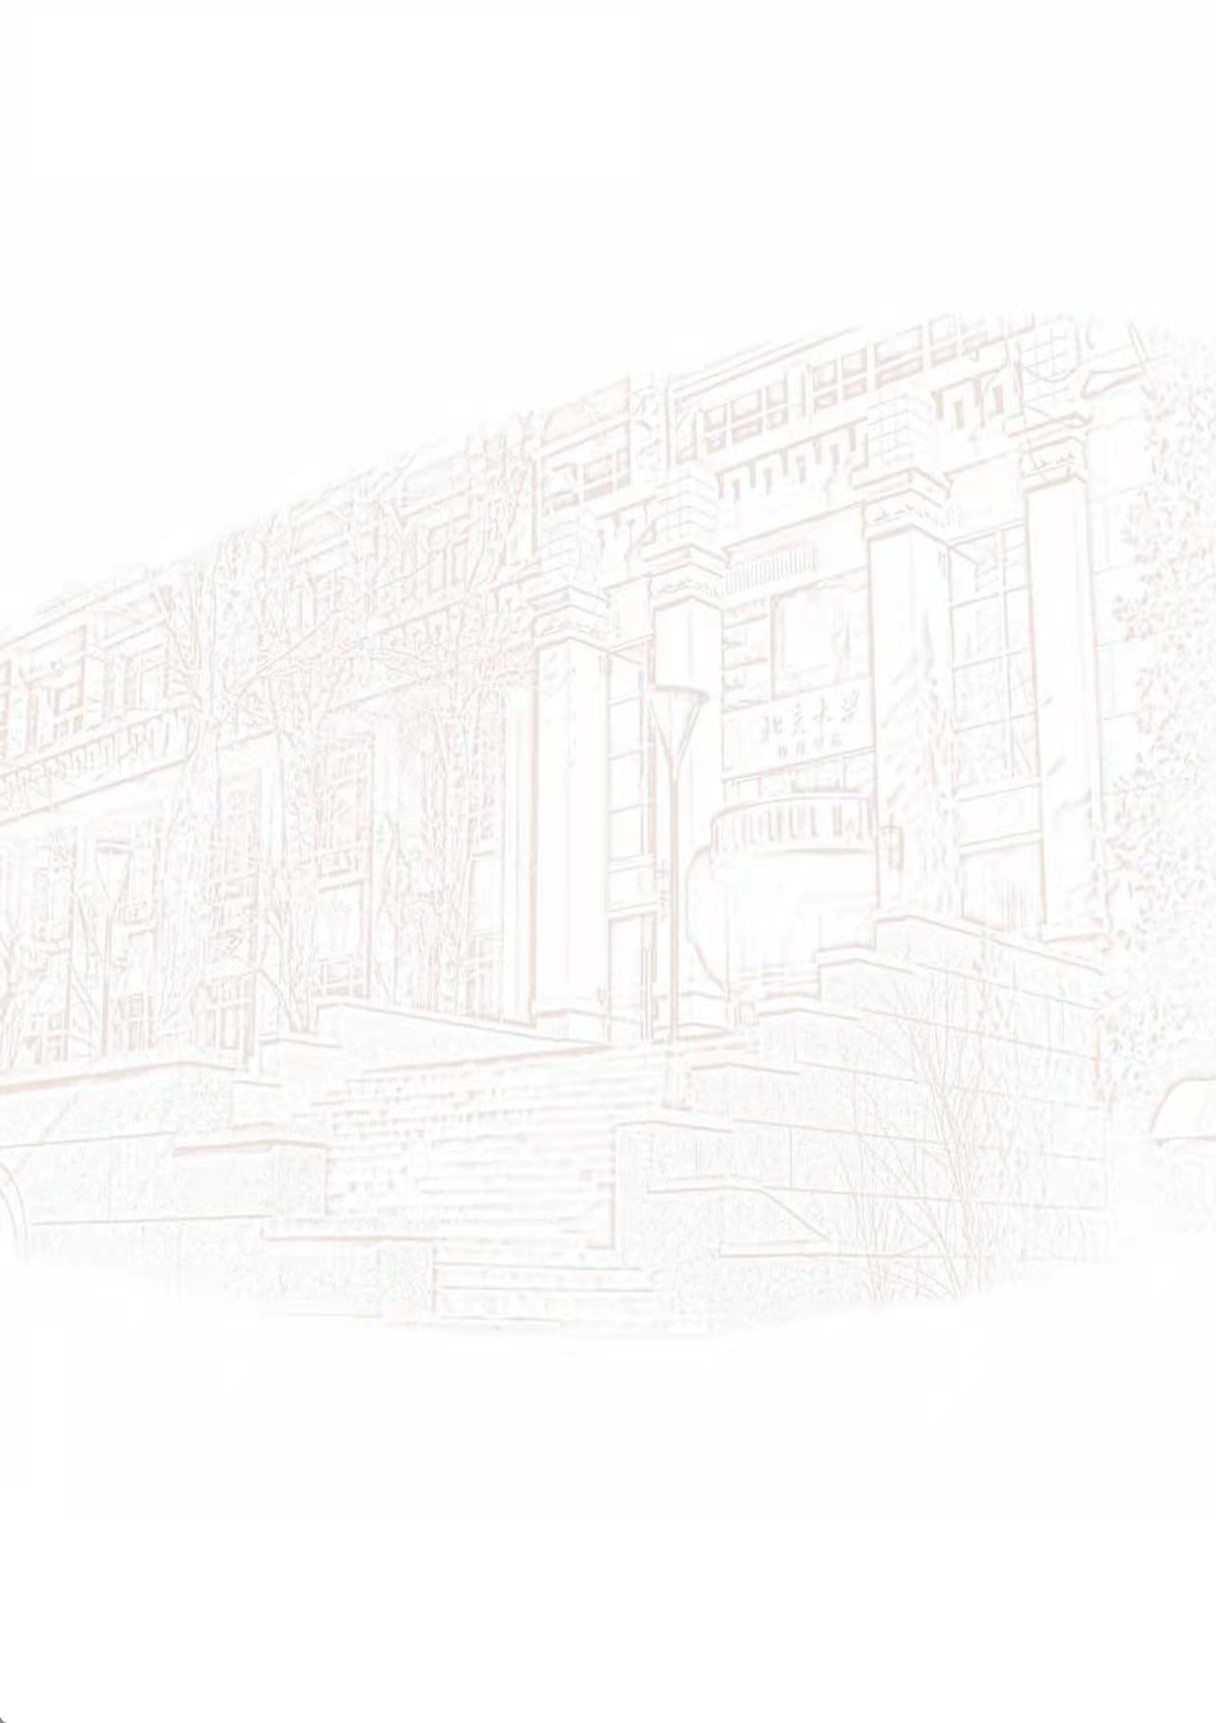
\includegraphics[width=\paperwidth, height=\paperwidth, keepaspectratio]{pic/phy.jpg}}}
\addbibresource{ref.bib}
\renewcommand*{\bibfont}{\zihao{5}\linespread{1.27}\selectfont}
%\usepackage{background}
%\backgroundsetup{scale=1,angle=0,opacity=1,contents={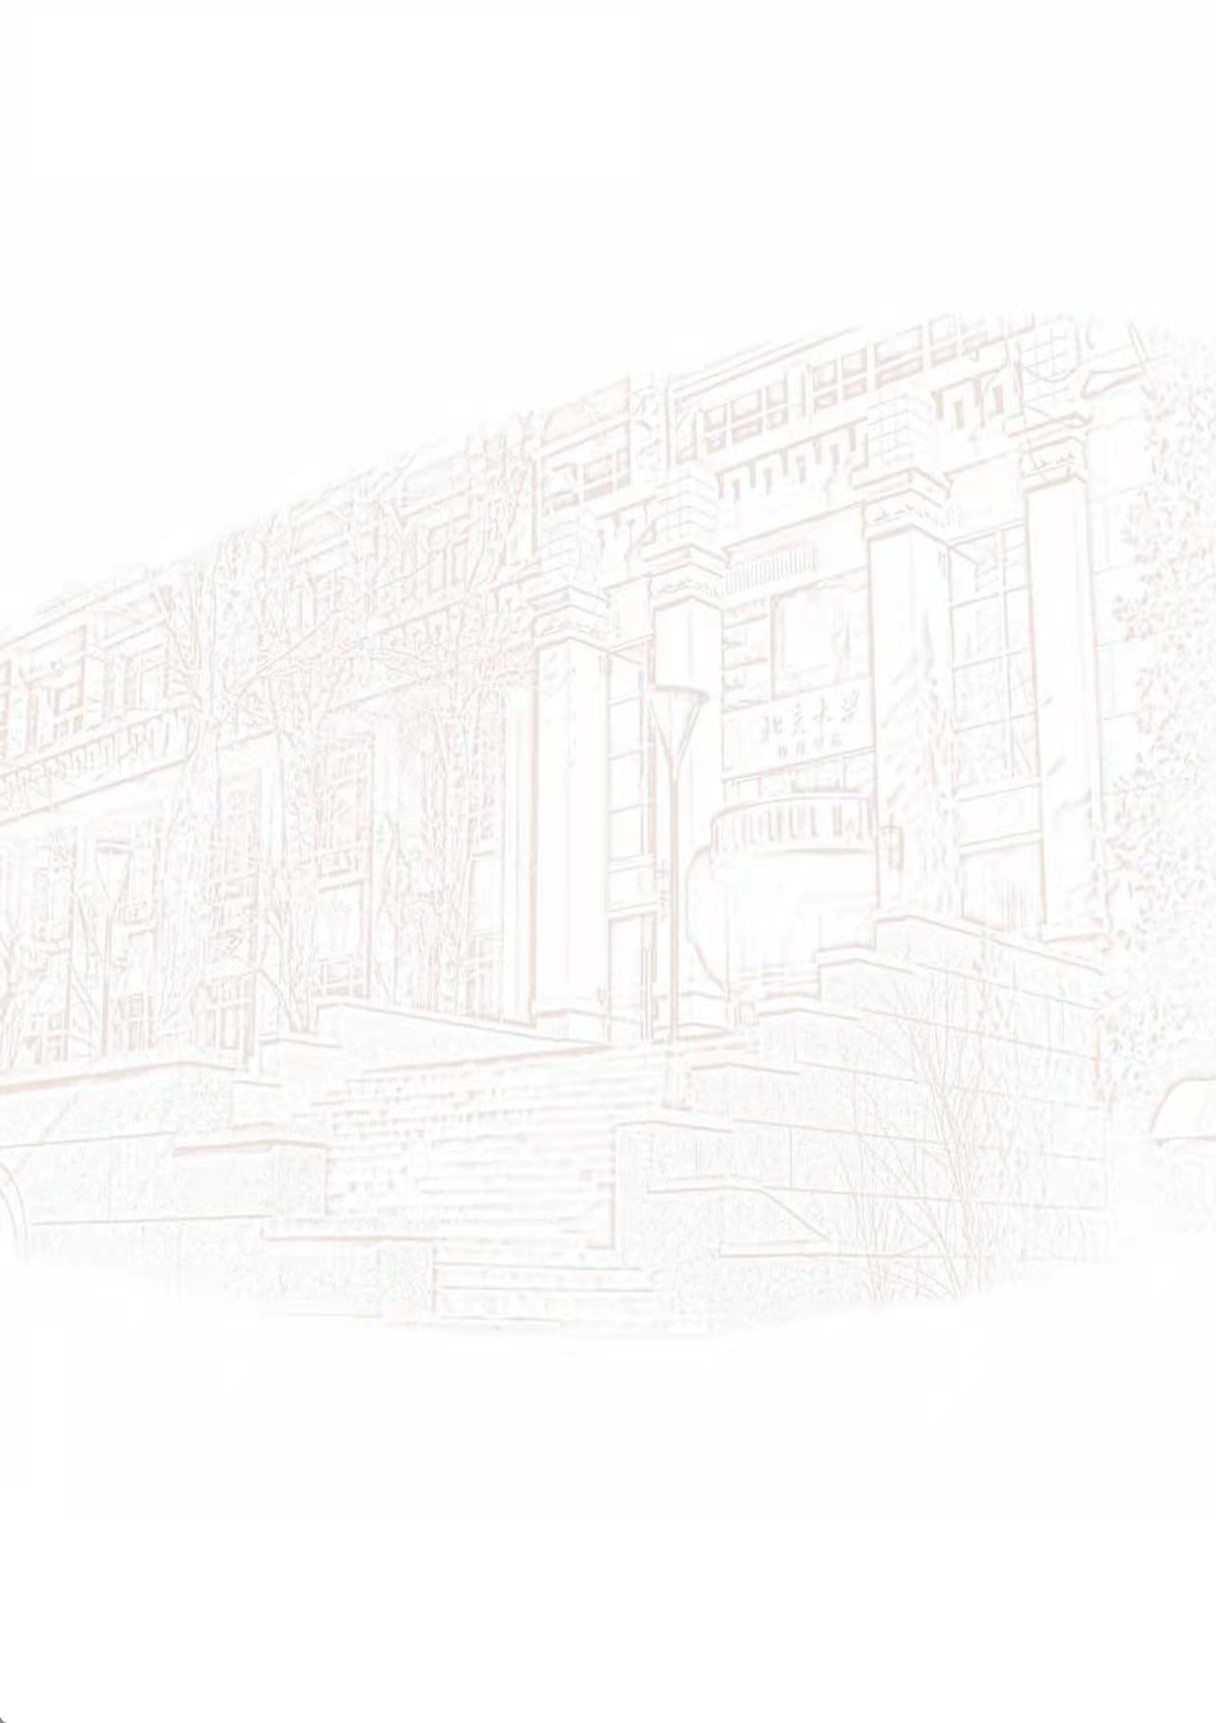
\includegraphics[width=\paperwidth, height=\paperwidth, keepaspectratio]{pic/phy.jpg}}}
%\ctexset{punct=kaiming}
\setCJKmainfont[ItalicFont=FZKTK.TTF,BoldFont=FZXBSK.TTF]{FZSSK.TTF}
\setCJKsansfont[BoldFont=FZHTK.TTF]{FZXH1K.TTF}
\setCJKmonofont[ItalicFont=FZKTK.TTF]{FZFSK.TTF}
\newCJKfontfamily\FZSS{FZSSK.TTF}
\newCJKfontfamily\FZKT{FZKTK.TTF}
\newCJKfontfamily\FZFS{FZFSK.TTF}
\newCJKfontfamily\FZHT{FZHTK.TTF}
\setmainfont{TeX Gyre Termes}
\setsansfont{TeX Gyre Heros}[Scale=MatchLowercase]
\setmonofont{Ubuntu Mono}%[Scale=MatchLowercase]
\newfontfamily\lm{Latin Modern Roman}
\usepackage{unicode-math}
\setmathfont{TeX Gyre Termes Math}

\newcommand\pkg[1]{\textsf{#1}}
\newenvironment{csop}{\vskip\topsep\noindent\hspace{2em}\ttfamily\small\ignorespaces}{\vskip\topsep\par}
\usepackage{float}
\usepackage{booktabs,metalogo,siunitx,marginnote,manfnt,url}
\usepackage[unicode]{hyperref}
\hypersetup{pdfstartview=XYZ,hidelinks,pdfcreator=XeTeX Output,pdfauthor=吴熙楠,
pdftitle=phyasgn文档类}
\usepackage{geometry,fancyhdr}
\geometry{left=3cm,right=3cm,marginparwidth=4em}
\fancyhead[L]
{\begin{tabular}[b]{@{}l@{}}
  \hyperref{https://www.pku.phy.edu.cn/}{}{}{
\includegraphics[height=2em]{phylogo.pdf}}
\end{tabular}}
\fancyhead[C]
{\begin{tabular}[b]{@{}c@{}}
  \large 
  基于饱和吸收的远场超分辨成像
  \\[-2pt]
  {\scriptsize 姓名:~吴熙楠\quad 学号:~1900011413}
\end{tabular}
}

\usepackage{shortvrb,fancyvrb}
\MakeShortVerb|
\fvset{xleftmargin=2em,fontsize=\small}
\makeatletter
\ifx\l@nohyphenation\undefined
  \newlanguage\l@nohyphenation
\fi
\DeclareRobustCommand\meta[1]{%
  \ensuremath\langle
  \ifmmode \expandafter \nfss@text \fi
  {%
    \rmfamily\itshape
    \edef\meta@hyphen@restore
    {\hyphenchar\the\font\the\hyphenchar\font}%
  \hyphenchar\font\m@ne
  \language\l@nohyphenation
  #1\/%
  \meta@hyphen@restore
  }\ensuremath\rangle
}
\makeatother

\def\phyasgn{\pkg{phyasgn}}
\def\version{0.2 $\upbeta$}

\title{
  {基于饱和吸收的远场超分辨成像}\\[-8pt]
  {\normalsize ——几何光学与光学仪器阅读报告}
}
\author{吴熙楠}
\date{\today}
\begin{document}
\maketitle

\begin{abstract}
在课堂上我们学到了许多时间分辨与空间分辨的相关技术,如:光电子显微镜,条纹相机,近场扫描显微镜,原子力显微镜等。对于空间分辨部分,如果想要得到远场的光学成像,不可避免的会出现分辨率衍射极限的问题,限制了远场光学显微镜的进一步应用。但是如果利用材料的非线性饱和吸收效应,可以制造出超过分辨率衍射极限的显微镜,这样的显微镜不仅能进行横向的超分辨成像,也能进行轴向的超分辨成像。
\end{abstract}

\tableofcontents

\section{引言}
远场光学显微镜作为一种无创性工具在生物或凝聚态领域已被广泛使用,但空间分辨率光学衍射极限的限制,即使目前光学共焦系统有很大的进步,光学显微镜的空间分辨率在横向和轴向位置仍然分别限制在$\sim$250 nm和$\sim$ 500 nm。为了克服这一障碍,科学家们利用扫描金属光栅近场的倏逝波,首次获得了亚波长的空间分辨率\cite{ash1972super},之后扫描近场显微镜开始蓬勃发展,由于倏逝波不受到衍射极限的限制,分辨率取决于孔径与倏逝波的性质,目前已经能达到20nm的分辨率\cite{doi:10.1063/1.336848},但此项技术受到工程方面的困难目前研究较为缓慢;同时也有科学家将扫描近场显微镜与原子力显微镜结合利用近场倏逝波研究材料性质\cite{BETZIG1986269},但由于扫描针尖的问题以及不能进行轴向的成像,难以应用于所有样品。
\par 因此,实际上研究远场超分辨率成像显微镜也是目前研究的一个方向,尤其是无标签染色的显微镜能尽可能减少对于样品的损坏,对于生物领域以及材料科学领域的研究有重大应用。目前,超分辨远场光学显微镜这方面的研究很多,下面将介绍一种不依赖于荧光的远场光学显微镜,它是基于Pump-Probe过程,但加入了另一束强环形激光以使得环形区域材料达到非线性饱和吸收,从而探测脉冲对材料的调制只发生在环形区域中心,这个区域可以远小于光学衍射极限,因此达到超分辨率成像的效果。
\par 本文作为阅读报告将简单介绍此类显微镜的原理,以及文献\cite{doi:10.1021/acs.nanolett.1c00403,wang2013far,Bi:20,doi:10.1021/acsphotonics.9b01821}中的实验结果,最后对其特点做总结与展望。
\section{原理}
我们考虑一个简单的双能级系统,如图\ref{1}所示:
	\begin{figure}[!h]
	\centering
	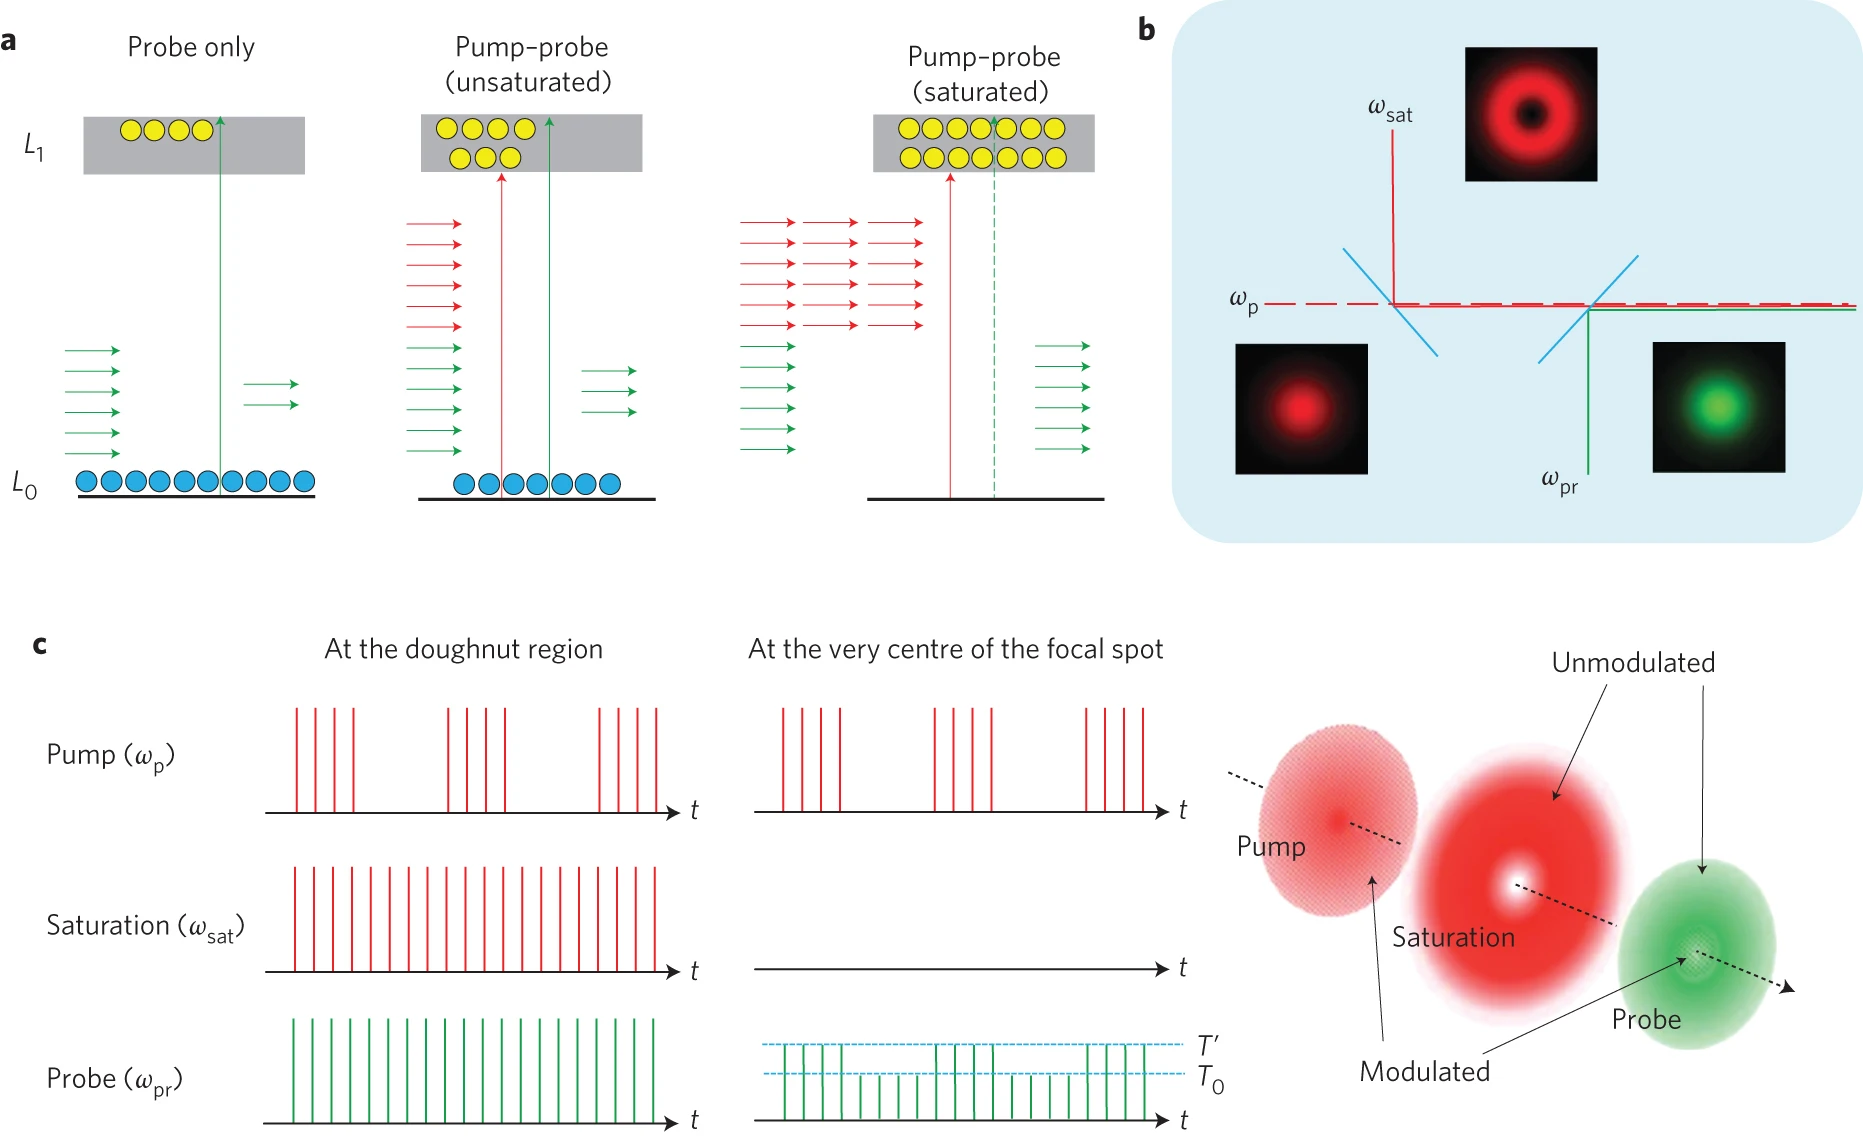
\includegraphics[width=.95\linewidth]{pic/1.png}
	\caption[饱和吸收显微镜原理]{饱和瞬态吸收显微镜原理\cite{wang2013far}}\vspace{1ex}
	\label{1}
	\end{figure}
    \par 如图\ref{1}a所示,吸收$\omega_{pr}$频率的探测光子,能将系统从$L_{0}$激发到$L_{1}$,从而导致透射率下降,但当我们引入$\omega_{p}$的泵浦光场时,泵浦激励会消耗$L_{0}$的布居数数量,从而相应地减少对探测光的吸收。当泵浦光场的强度足够高时,它通过耗尽$L_{0}$处的布居数或填充$L_{1}$能态使电子跃迁饱和。最后的结果就是探测光子的瞬态吸收被抑制。基于这一原理,饱和瞬态吸收显微镜被设计为通过共线性添加与泵浦光波长相同但强度更高的非调制饱和光束($\omega_{sat}$),将探测面积减小到Pump-Probe显微镜的衍射极限以下(如图\ref{1}b所示)。在饱和光束强度较高的环形区域,由于电子跃迁的饱和,探测光的传输保持不变,就如同材料透明一样。在这种条件下,Pump-Probe调制转移只发生在饱和光束强度接近于零的焦点中心(如图\ref{1}c)。通过对三束共线对准的光束在样品上同时进行光栅扫描,可以获得超分辨率图像。
    \par 其中对于大部分的饱和吸收材料,其可见光与近红外区域,探测光的透过率随泵浦光功率的变化关系如式\eqref{eq1}:
    \begin{equation}
    T_{pr}=T_{0}+\dfrac{hI_{p}}{1+I_{p}/I_{0}}
    \label{eq1}
    \end{equation}
    \par 式\eqref{eq1}中,$T_{pr}$为探测光束的透过率,$T_{0}$为不存在泵浦能量的探测光束的透过率,$I_{p}$为泵浦光束的功率密度,$h$和$I_{0}$分别为表征调制透过系数和饱和吸收功率密度的常数。Pump-Probe测量的对比来自于泵浦光开、关状态下探头透过率的差值,可以推导为式\eqref{eq2}:
    \begin{equation}
    \Delta T_{pr}=\dfrac{hI_{p}}{1+I_{p}/I_{0}}
    \label{eq2}
    \end{equation}
    \par 当我们加入饱和光束$I_{sat}$时,透过率变化可写为式\eqref{eq3}:
    \begin{equation}
    \Delta T_{pr}^{\prime}=\dfrac{h(I_{p}+I_{sat})}{1+(I_{p}+I_{sat})/I_{0}}-\dfrac{hI_{sat}}{1+I_{sat}/I_{0}}
    \label{eq3}
    \end{equation}
    \par 当我们考虑$I_{p}<<I_{0}$时,可以将式\eqref{eq3}近似为如下式\eqref{eq4}:
    \begin{equation}
        \Delta T_{pr}^{\prime}=\dfrac{hI_{p}}{1+I_{sat}/I_{0}}
        \label{eq4}
        \end{equation}
     \par 由式\eqref{eq4}可以看出Pump-Probe信号在高强度饱和波束的存在下被抑制,当$I_{sat} = I_{0}$时,Pump-Probe信号下降到一半。
\section{实验装置}
实验装置如图\ref{2}所示,其中图\ref{2}中右上插图为发送到SLM的螺旋相图案,以产生饱和光束的圆环形的输出。左下角插图为使用20 nm 的ZnO纳米晶体的二次谐波成像测量的饱和光束的PSF。
\begin{figure}[!h]
	\centering
	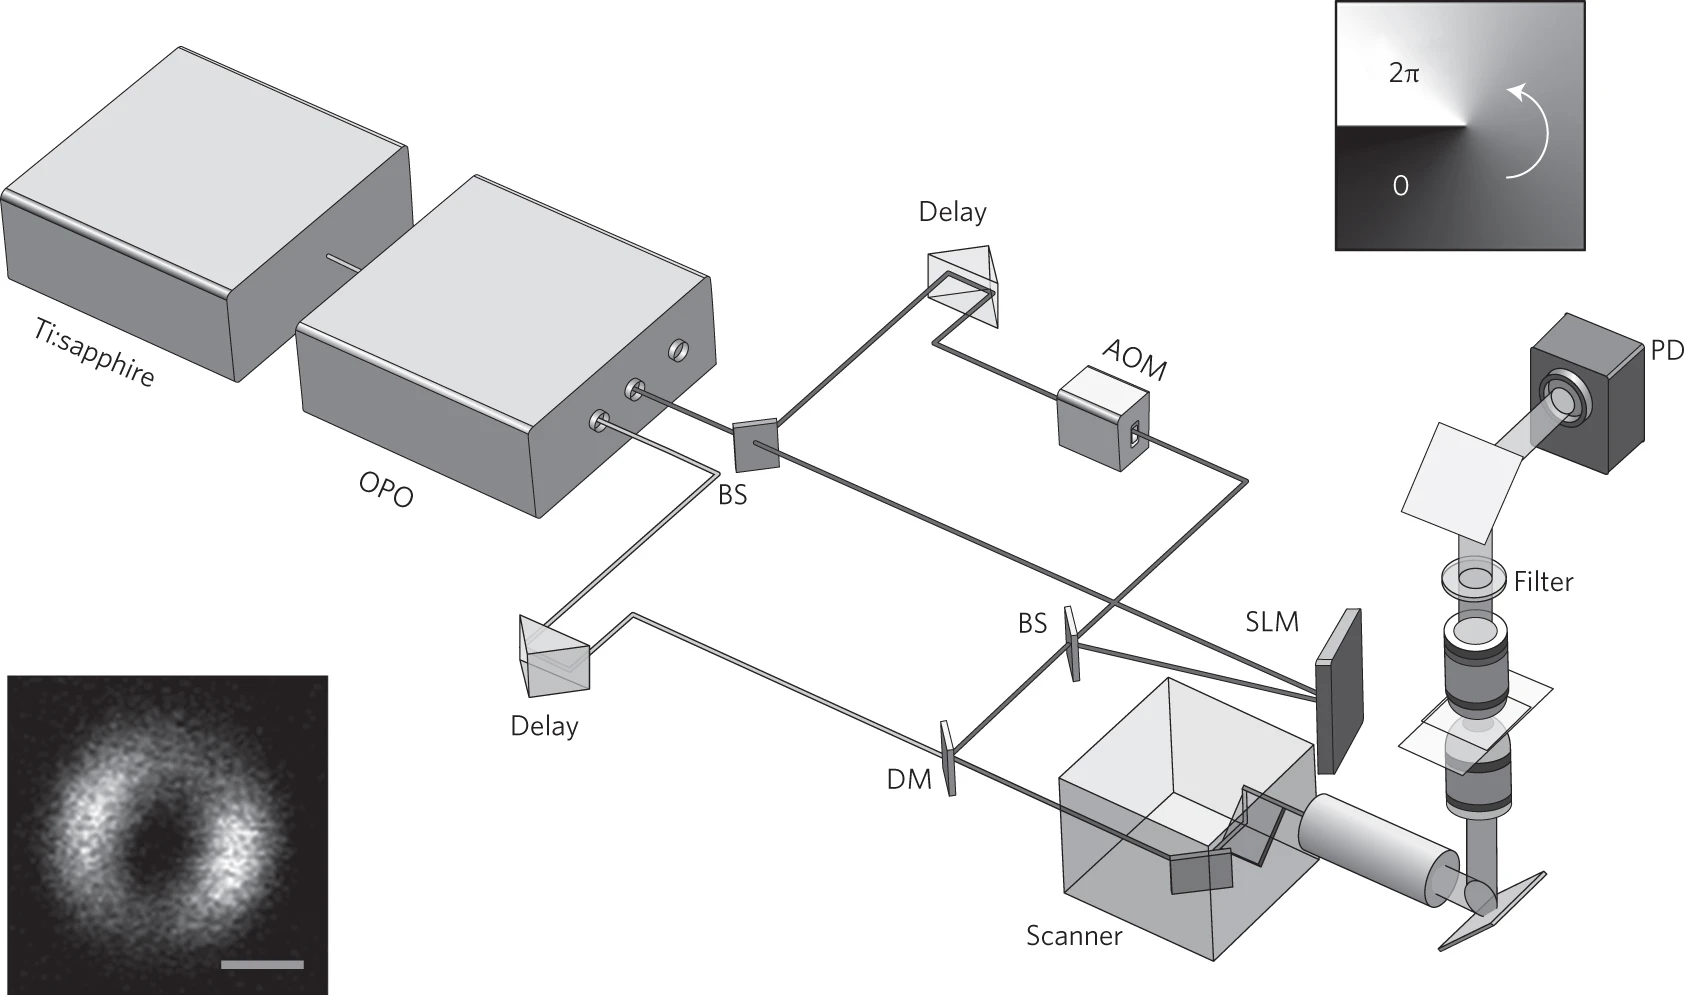
\includegraphics[width=.95\linewidth]{pic/2.png}
	\caption[饱和吸收显微镜原理]{饱和吸收显微镜实验装置示意图\cite{wang2013far},其中,OPO,光学参数振荡器;AOM,声光调制器;BS, 分光镜;SLM,空间光调制器;PD,光电二极管;DM,二向色镜。}\vspace{1ex}
	\label{2}
	\end{figure}
    \par 在此实验装置中,830 nm激光器泵浦了一个光学参量振荡器,提供1064 nm的输出,脉冲宽度约为260 fs。将1064nm光束分为两臂,分别作为泵浦光和饱和光。泵浦光束由声光调制器调制。饱和光束被定向到一个纯相位SLM,通过输入一个从$0-2\pi$的螺旋相位斜坡生成一个圆环形状(探测光只对中心位置调制作出响应)。应用继电器光学元件将圆环形光束投射到物镜上。830nm光束用作探测光,并与泵浦光和饱和光束共线组合。将三束束送至激光扫描显微镜,并通过物镜聚焦到样品上。透射的探测光由另一个物镜收集,并由光电二极管检测,然后由谐振放大器检测。使用锁相放大器在调制频率下提取探测信号。
    \par 参考另一篇文献\cite{doi:10.1021/acs.nanolett.1c00403}的实验装置图(图\ref{3}),可见其实验装置图是差不多的,其实验装置运行过程不再赘述。
\begin{figure}[!h]
	\centering
	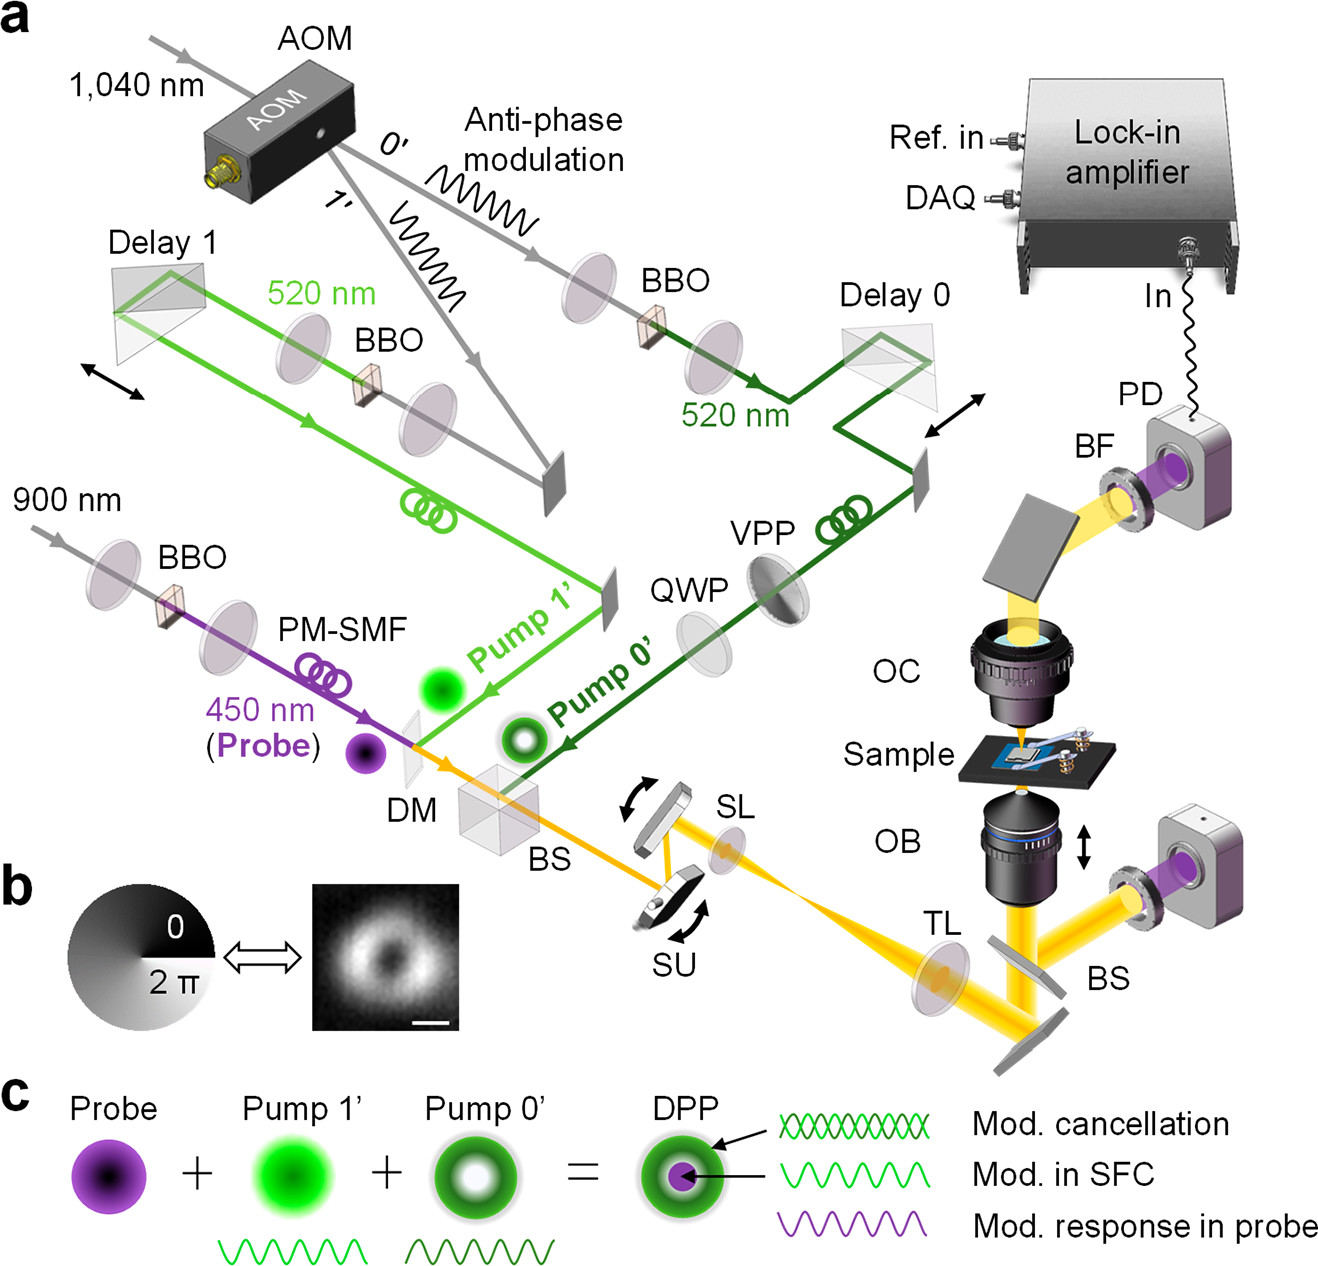
\includegraphics[width=.8\linewidth]{pic/3.png}
	\caption[饱和吸收显微镜原理]{饱和吸收显微镜实验装置示意图\cite{doi:10.1021/acs.nanolett.1c00403},其中,AOM:声光调制器;VPP:涡旋相位板;QWP:1/4波片;PM-SMF:保偏振单模光纤;DM:分色镜;BS:分束器;SU:扫描单元;SL:扫描透镜;TL:管透镜;OB:目标;OC:油冷凝器;BF:带通滤波器;PD:光电二极管;DAQ:数据采集器。}\vspace{1ex}
	\label{3}
	\end{figure}
    \par 值得注意的是,过于高功率的饱和光束可能会超过样品的损伤阈值,因此我们应该以低于样品损伤阈值的饱和光束进行实验。
\section{实验结果}
以下分别列出四篇文献中利用饱和瞬态吸收的方法提高分辨率的例子如下。
\begin{figure}[!h]
	\centering
	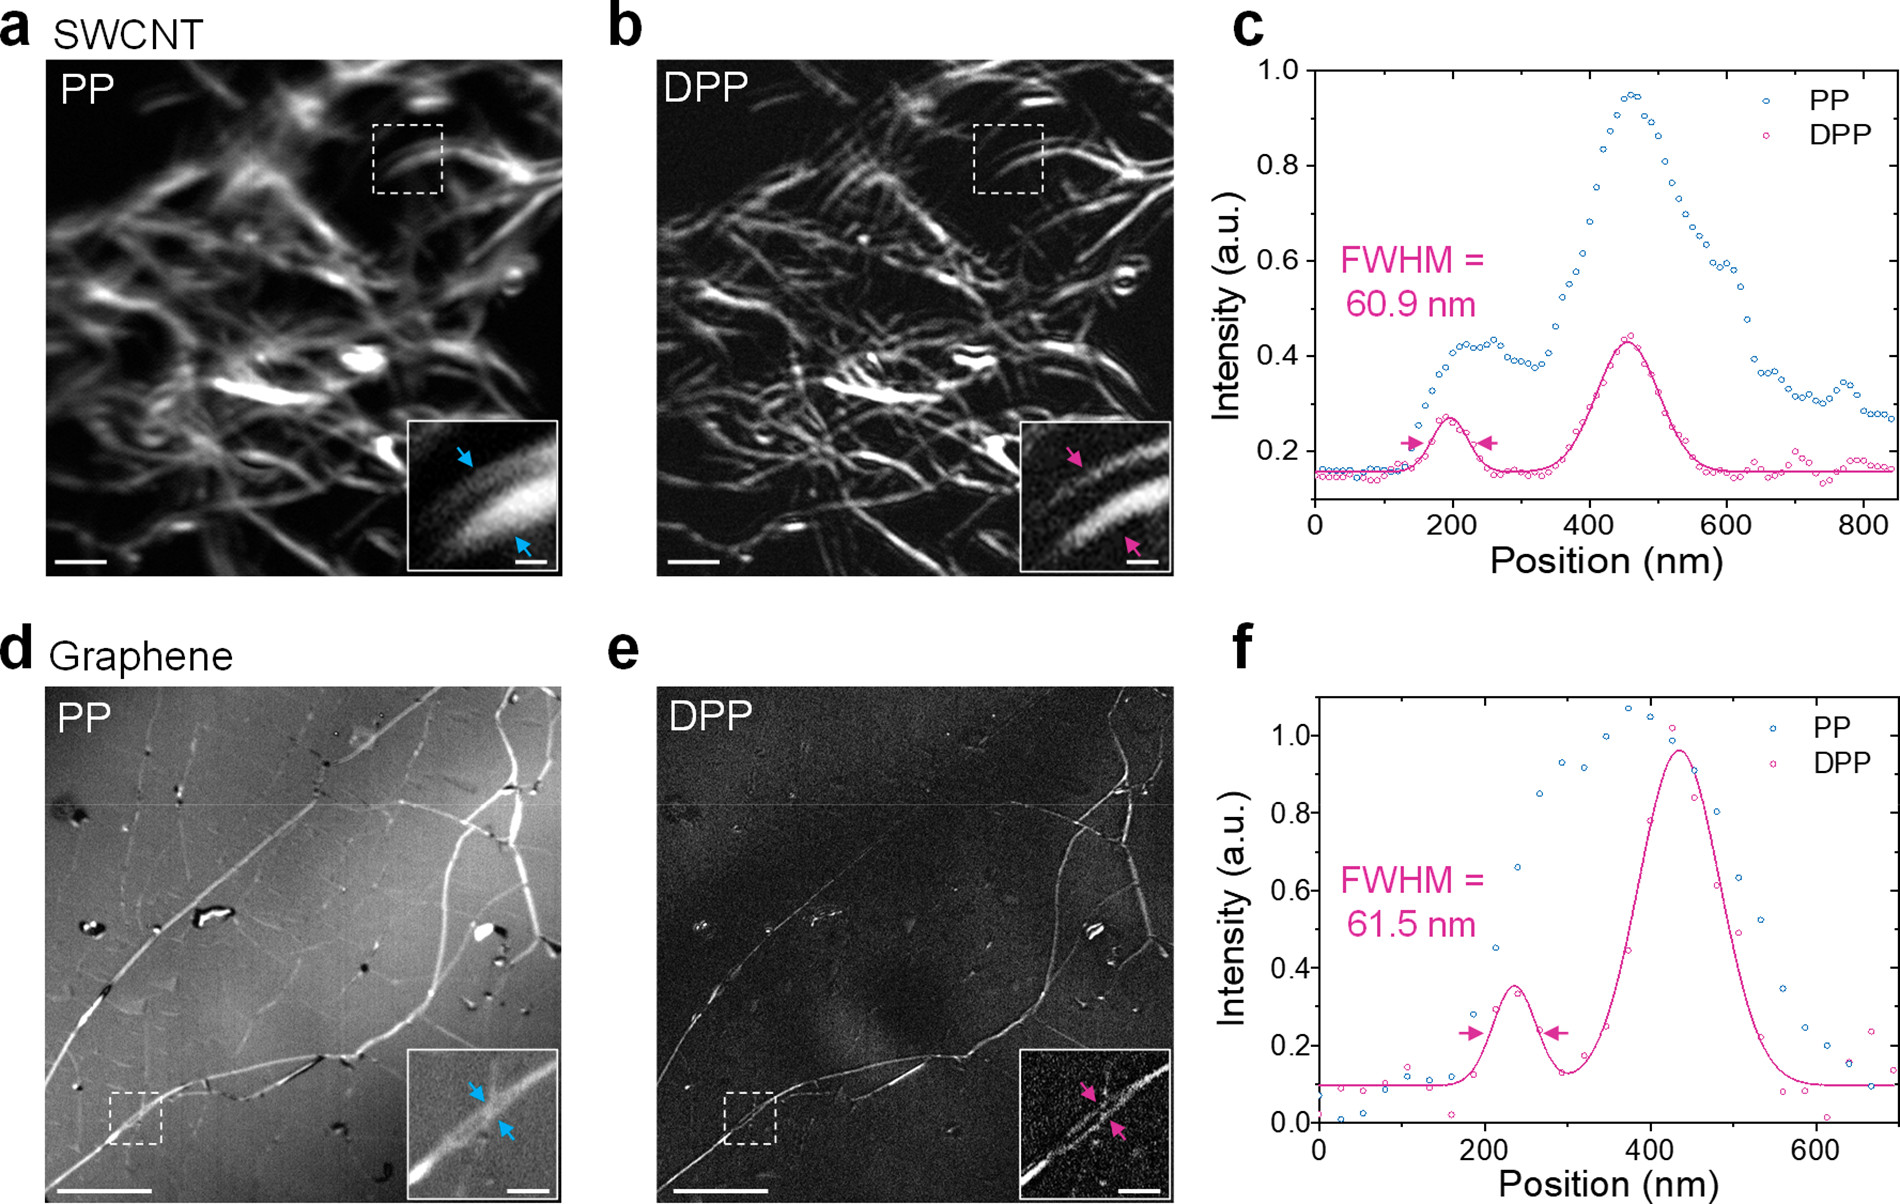
\includegraphics[width=.9\linewidth]{pic/4.png}
	\caption[饱和吸收显微镜原理]{普通Pump-Probe方法与饱和吸收Pump-Probe方法对单壁碳纳米管与单层石墨烯进行成像对比\cite{doi:10.1021/acs.nanolett.1c00403}}\vspace{1ex}
	\label{4}
	\end{figure}
    \par 由图\ref{4}可以看出,饱和吸收的Pump-Probe方法相比普通的不增加饱和光束的Pump-Probe方法而言,成像质量与分辨率有了明显的提高,普通方法分辨率还停留在衍射极限300nm左右,而饱和吸收Pump-Probe方法已经可以达到低于100nm的分辨率。
\begin{figure}[!h]
	\centering
	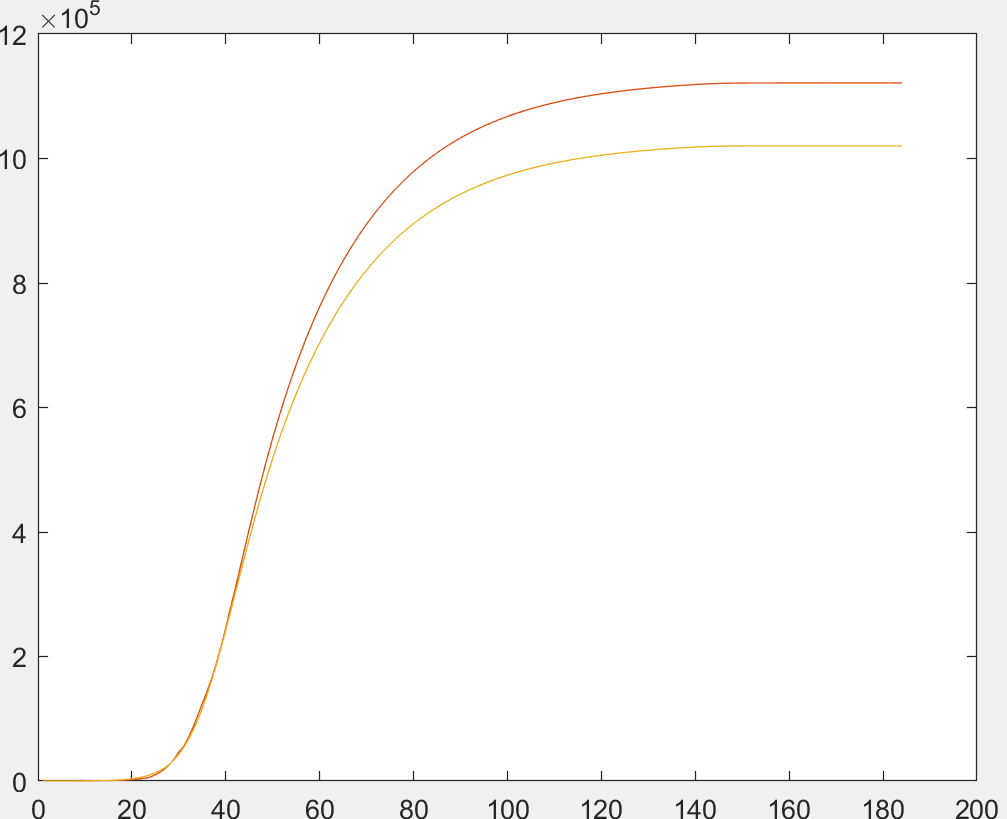
\includegraphics[width=.9\linewidth]{pic/5.png}
	\caption[饱和吸收显微镜原理]{饱和吸收显微镜成像与SEM成像对比\cite{doi:10.1021/acs.nanolett.1c00403}}\vspace{1ex}
	\label{5}
	\end{figure}
    \par 由此图\ref{5}中饱和吸收显微镜与SEM成像对比图可以看出,SEM的分辨率还是要好于饱和吸收显微镜的,但是其已经能超过光学衍射极限的分辨率,并且由SEM扫描图来看,图像的准确度也在不错的水平。
\begin{figure}[!h]
	\centering
	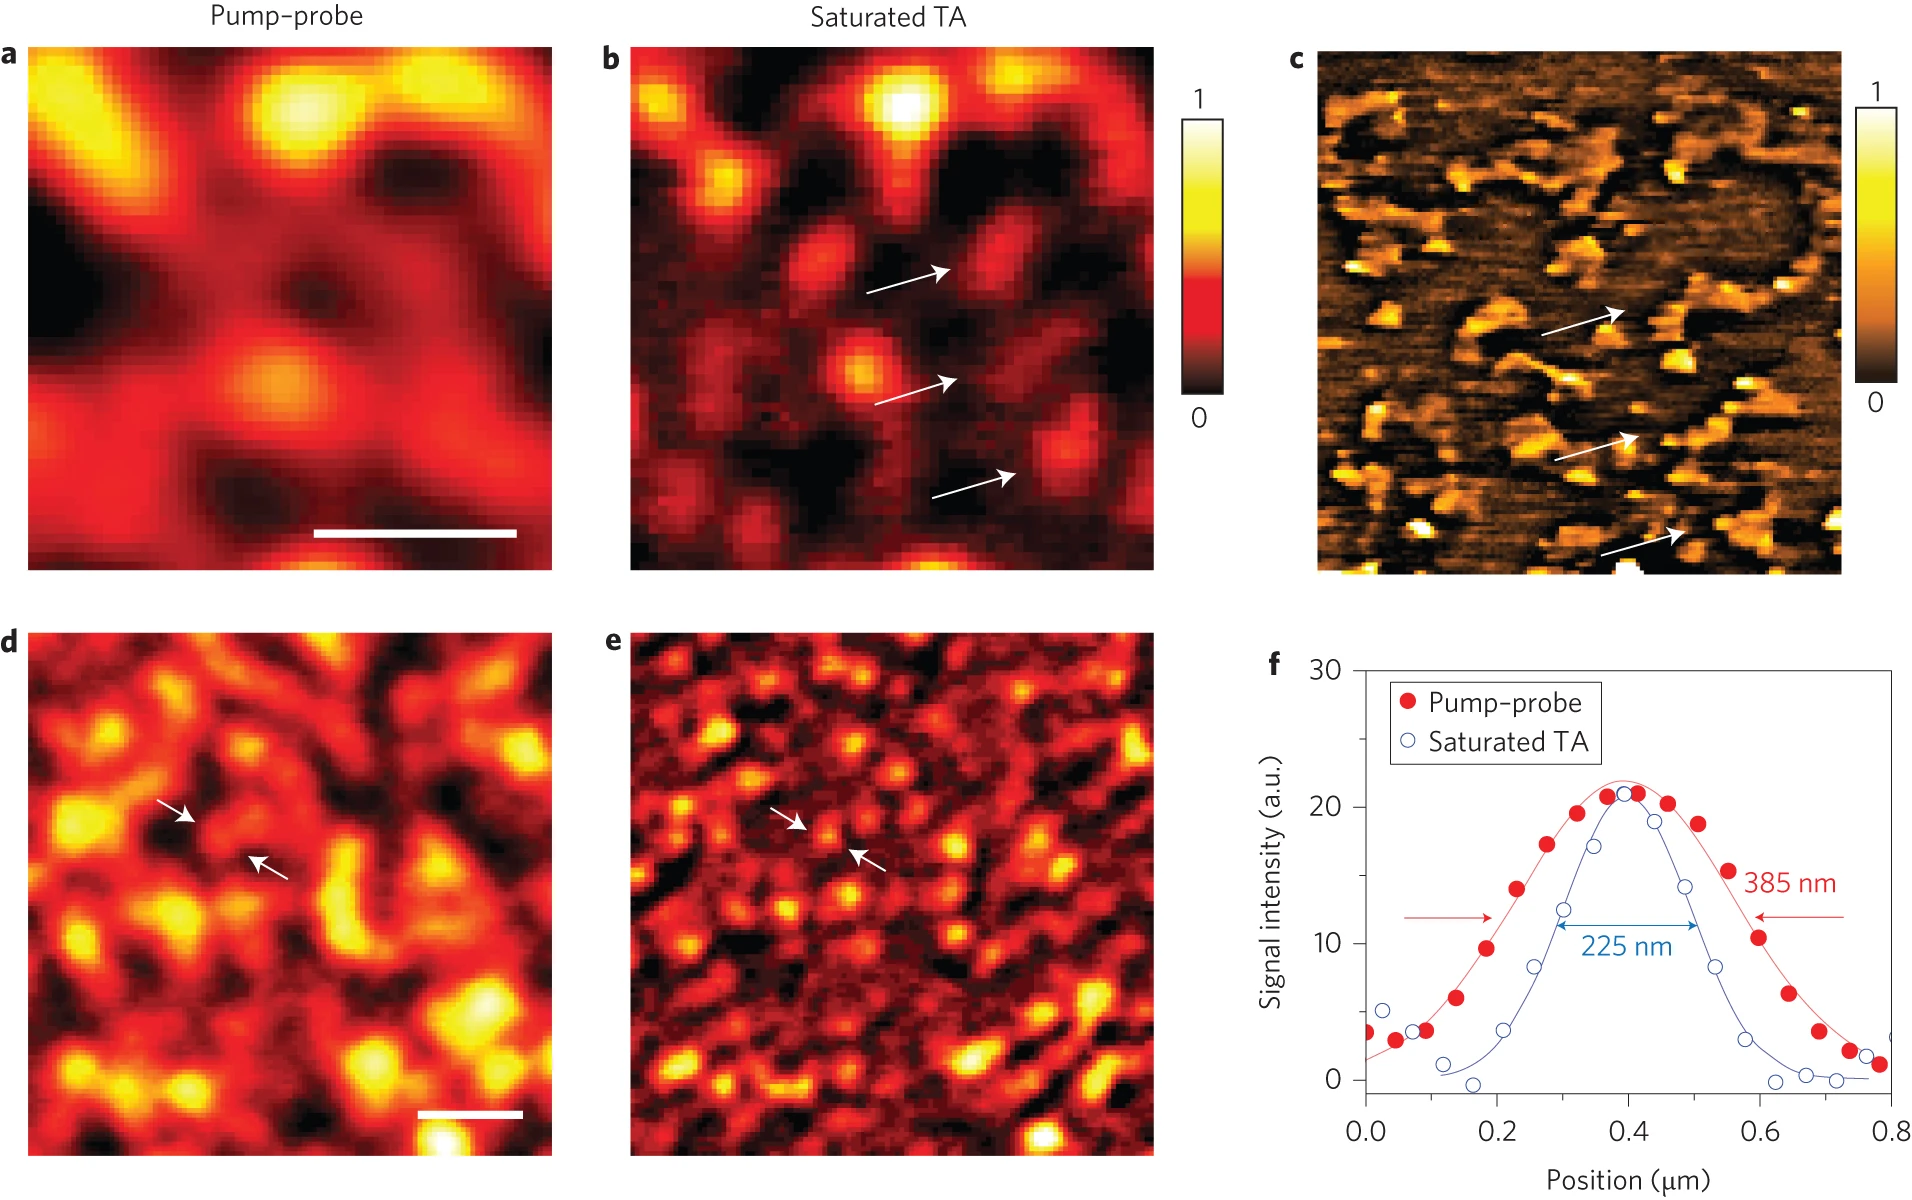
\includegraphics[width=.9\linewidth]{pic/6.png}
	\caption[饱和吸收显微镜原理]{饱和吸收显微镜成像与普通Pump-Probe显微镜以及AFM成像对比\cite{wang2013far}}\vspace{1ex}
	\label{6}
	\end{figure}  
    \par 由图\ref{6}可以看出,和图\ref{4}与图\ref{5}相同,饱和吸收显微镜成像质量与分辨率显著高于普通Pump-Probe显微镜成像,并且与近场的AFM扫描成像进行对比,发现其成像真实度很高。  
\begin{figure}[!h]
	\centering
	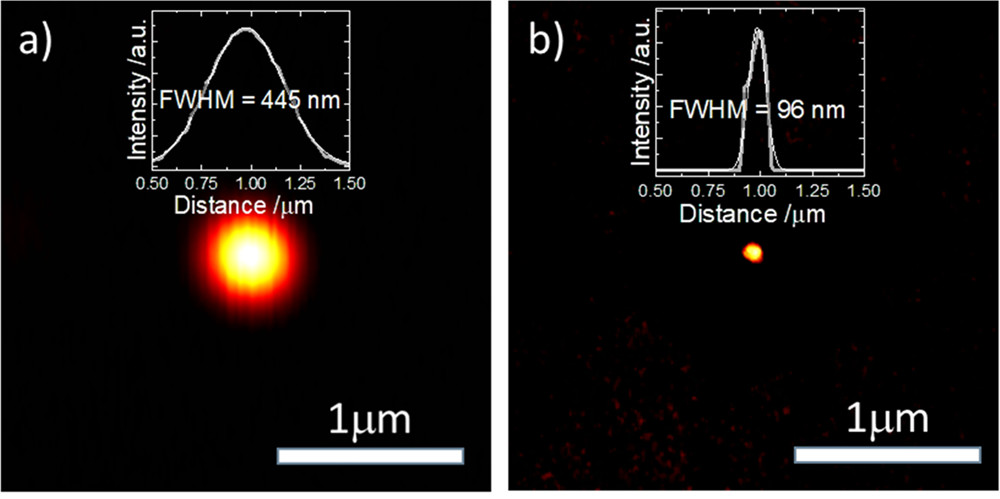
\includegraphics[width=.9\linewidth]{pic/7.png}
	\caption[饱和吸收显微镜原理]{饱和吸收显微镜成像与普通Pump-Probe显微镜成像对比\cite{doi:10.1021/acsphotonics.9b01821}}\vspace{1ex}
	\label{7}
	\end{figure}  
    \par 图\ref{7}与图\ref{4}相同,饱和吸收显微镜成像质量与分辨率能够低于100nm,显著优于普通Pump-Probe显微镜能达到的衍射极限400nm。
\begin{figure}[!h]
	\centering
	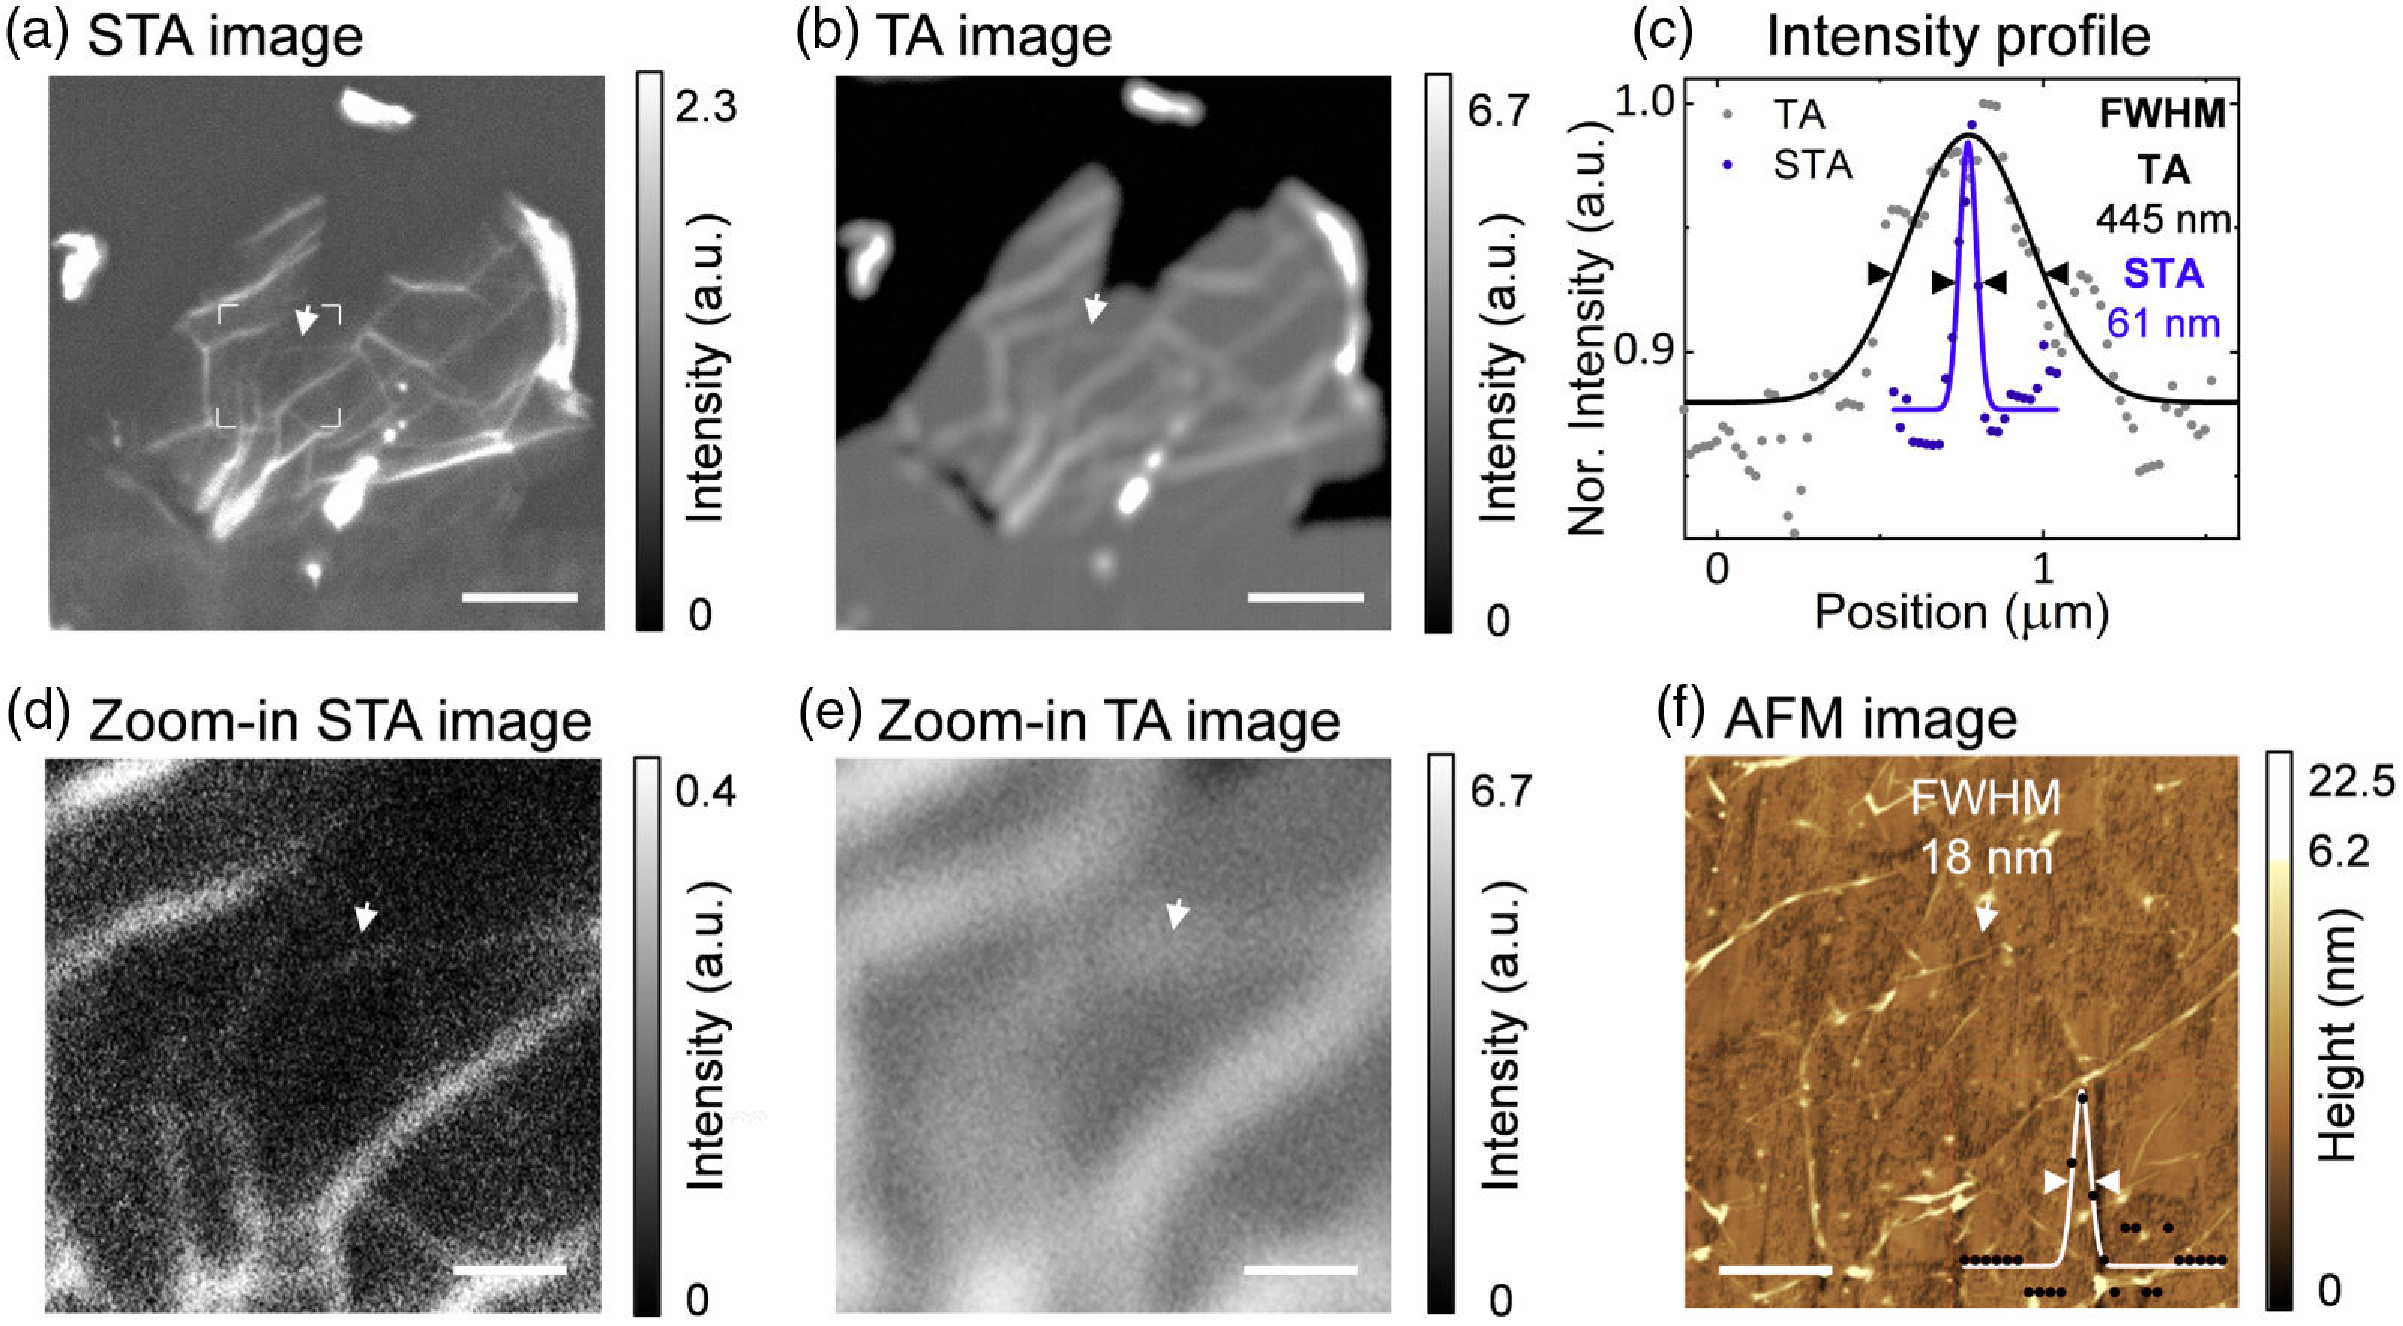
\includegraphics[width=.9\linewidth]{pic/8.png}
	\caption[饱和吸收显微镜原理]{饱和吸收显微镜对石墨烯成像与普通Pump-Probe显微镜以及AFM成像的对比\cite{Bi:20}}\vspace{1ex}
	\label{8}
	\end{figure} 
    \par 图\ref{8}与以上如图\ref{6}相同,均在近红外的泵浦光束与探测光书情况下实现了低于100nm分辨率的超分辨成像,并且与AFM成像进行了对比,表明其成像是真实可靠的。
    \par 从上述四篇文献的实验结果数据中可以看出,饱和吸收显微镜确实能够实现远场光学的超分辨成像,其分辨率能够达到低于100nm,远低于普通显微镜的衍射极限,并通过SEM与AFM成像的对比可以看出,其成像有非常高的可信度。
\section{总结与展望}
从上述实验结果中我们可以看出,通过使用圆环形状的饱和激光,可以有效终止由泵浦和探测激光驱动的瞬态吸收过程,显微镜的空间分辨率可以提高到100nm以下(通过优化成像条件,例如通过应用较短的激发波长和以更快的扫描速度增加光损伤阈值,可以进一步提高分辨率),非常适合二维材料等具有饱和吸收性质的纳米材料的快速形态和电学的表征,大大降低了对样品制备和成像环境的要求,与之前报道的基于扫描隧道显微镜或近场扫描光学显微镜的Pump-Probe方法相比,这种方法的成像速度更快。此外,饱和瞬态吸收显微镜固有的光学切片能力使三维成像的横向分辨率低于衍射极限,同时通过应用z方向的圆环光束,也可以在轴向上提高分辨率,同时也不需要标记染色等操作,这些优势为在生物环境或功能材料内部研究纳米结构提供了新的机会。这种远场光学显微镜在未来可能将部分取代AFM、SEM和NSOM,用于材料科学和生物学中纳米结构的高分辨率成像和识别。
\printbibliography[heading=bibintoc]
\end{document}